%%%%%%%%%%%%%%%%%%%%%%%%%%%%%%%%%%%%%%%%%%%%%%%%%%%%%%%%%%%%
\documentclass[11pt,a4paper]{article}
\usepackage[a4paper,width=17cm,vmargin={2cm,2cm}]{geometry}
\usepackage{microtype}
\usepackage[style=verbose-inote,doi=false,sortcites=true, block=space]{biblatex}
\usepackage{fancyhdr}
\usepackage{graphicx}
\usepackage{amssymb}
\usepackage{mathrsfs}
\usepackage{amsmath}
\usepackage{amsfonts}
\usepackage{multirow}
\usepackage{eurosym}
\usepackage{dcolumn}
\usepackage{booktabs}
\usepackage{multirow}
\usepackage{enumitem}
\usepackage{hyperref}
\usepackage{framed}


%%%%%%%%%%%%%%%%%%%%%%%%%%%%%%%%%%%%%%%%%%%%%%%%%%%%%%%%%%%%
%% HEADERS 
\setlength{\headheight}{1cm}
\setlength{\headsep}{0.5cm}
\pagestyle{fancyplain}
\fancyhf{}
\lhead{\fancyplain{}{\sc G\'omez-Cadenas}}
\chead{\fancyplain{}{Part B}}
\rhead{\fancyplain{}{\sc PETALO}}
\cfoot{\thepage}
\renewcommand{\headrulewidth}{0pt} % remove lines
\renewcommand{\footrulewidth}{0pt}

%%%%%%%%%%%%%%%%%%%%%%%%%%%%%%%%%%%%%%%%%%%%%%%%%%%%%%%%%%%%
%% Hack to make math formulas bold in section titles
\makeatletter
\DeclareRobustCommand*{\bfseries}{%
  \not@math@alphabet\bfseries\mathbf
  \fontseries\bfdefault\selectfont
  \boldmath
}
\makeatother


%%%%%%%%%%%%%%%%%%%%%%%%%%%%%%%%%%%%%%%%%%%%%%%%%%%%%%%%%%%%
\def\thesection{\bf \textsf{\alph{section}}}
%\def\thesubsection{\alph{subsection}}
\def\thesubsubsection{\thesubsection.\arabic{subsubsection}}

\bibliography{biblio}
\begin{document}
%\input{src/Commands.tex}

%%%%%%%%%%%%%%%%%%%%%%%%%%%%%%%%%%%%%%%%%%%%%%%%%%%%%%%%%%%%
%% HEADING AND COVER PAGE
\begin{center}
{\Large \bf \textsf{ERC Proof of Concept Grant 2015}} \\ \vspace{0.3cm}
{\Large \bf \textsf{Part B1}} \\ \vspace{0.3cm}
{\LARGE \bf \textsf{PETALO: A Positron Emission Tof Apparatus based in Liquid xenOn}}\\ \vspace{0.3cm}
\end{center}

\newpage

\section*{\bf \textsf{Section 1-- The idea -- Innovation potential (max 2 pages)}}
\subsection*{a. Succinct description of the idea to be taken to proof of concept}

%\input{srcPoc/Idea.tex}

\begin{figure}[!htbp]
	\centering
	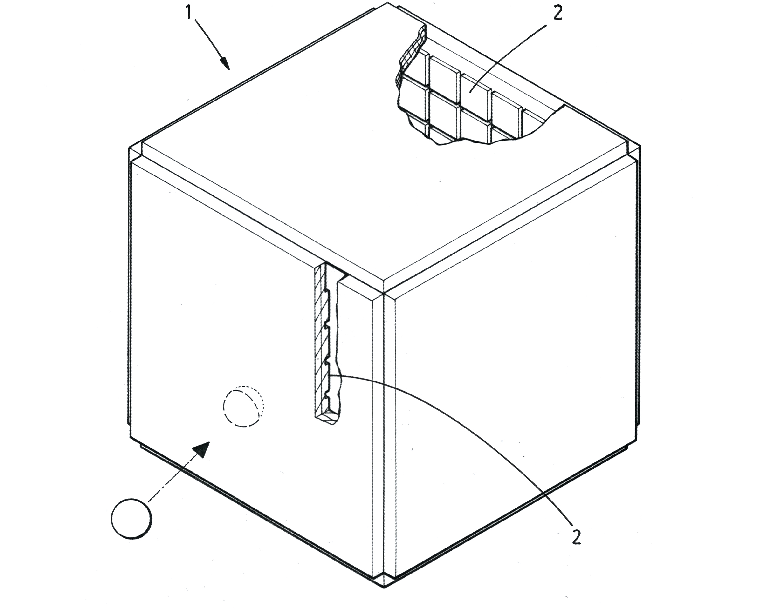
\includegraphics[scale=0.6]{img/LXSC2.pdf}
	%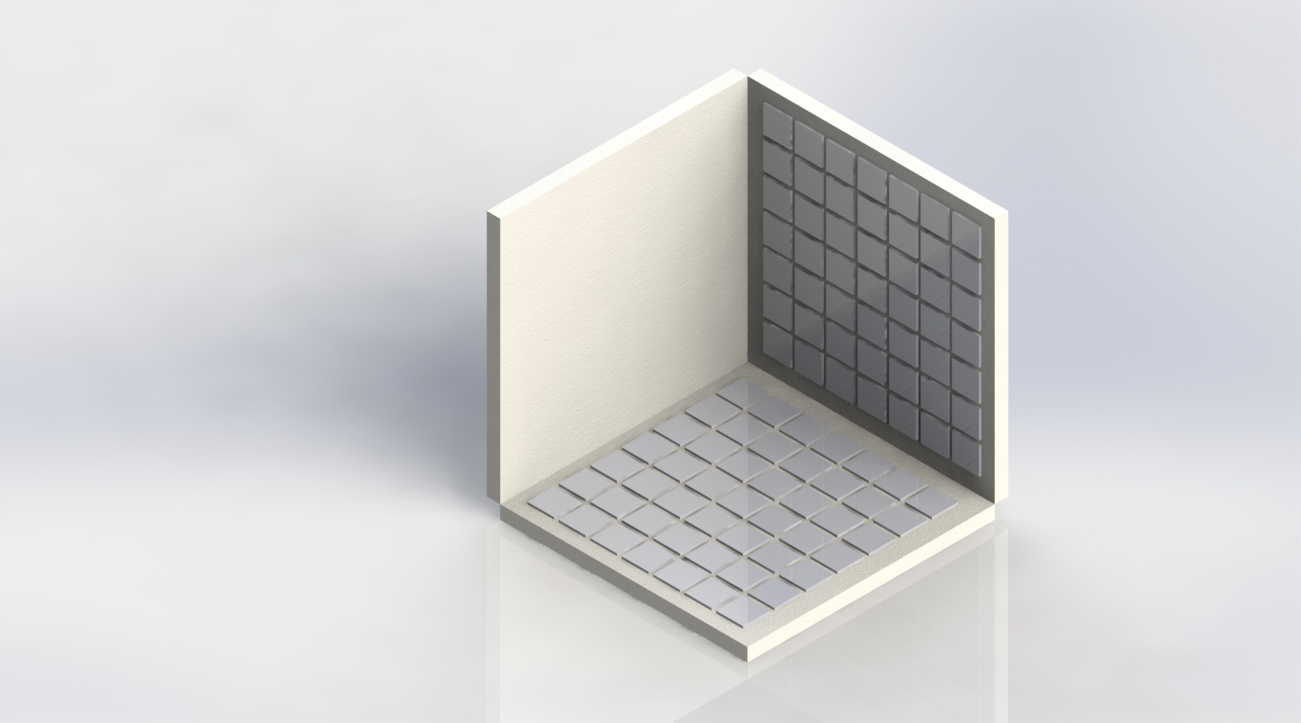
\includegraphics[scale=0.35]{img/box5open.jpg}
	\caption{\label{fig.box} The Liquid Xenon Scintillating Cell (LXSC) instruments the entry and exit faces of the box (relative to the photon line of flight) with silicon photomultipliers (SiPMs), coated with a wavelength shifter, tetraphenyl butadiene (TPB). The non-instrumented faces are covered by reflecting Teflon coated with TPB. The shape of the LXSC can be adapted to the application. }
\end{figure}

A PET (Positron-Electron Tomography) is a functional scan ---it does not show anatomic features--- whose main application is tumor diagnosis. It is based in the use of positron emitters radio-pharmaceuticals, injected into the patient prior to the scan. The emitted positrons slow down in the surrounding patient’s tissue, annihilating with atomic electrons to give two back-to-back 511 keV annihilation photons. By detecting the two photons in coincidence and measuring the coordinates of their interaction points in a detector, it is possible to define a line of response (LOR) along which the positron emitting source is located in the patient. A set of such intersecting lines allows 3D reconstruction of the source. 

%The main requirements for a PET detector are: (a) high photon detection efficiency ($\sim$ 80\% for each 511 keV gamma), (b) position resolution of a few millimeters, (c) time resolution to reduce the rate of false coincidences, (d) good energy resolution (10\% FWHM is typical in modern devices) to discriminate photons scattered in the patient and (e) a high count rate capability ($\sim10^6$~ s$^{-1}$ per cm$^2$~ of detecting surface). In addition, a PET system must have an angular acceptance as large as possible, which in turn requires a large axial (along the patient's body) coverage. However, due to the high cost of this devices, the axial size  of a PET is typically limited to 15-25 cm. 

Most modern PETs are built as rings using monolithic or segmented solid scintillating detectors (SSDs) readout by light sensitive detectors such as photomultipliers (PMTs), or Silicon Photomultipliers (SiPMs). Many of the high-end scanners use {\bf LSO/LYSO}, which is characterised by an {\bf attenuation length of 12 mm} to 511 keV photons, a  {\bf light yield of 29 photons per keV}, and a {\bf scintillation decay time of 40 ns}. This three parameters, essential for the performance of a PET scanner, result in an {\bf energy resolution} of, typically 10-15 \% FWHM; a {\bf spatial resolution} of the order of 1-3 mm for the transverse coordinates (typically achieved using segmented detectors readout by SiPMs) and 5-7 mm for the longitudinal coordinate ( in general not measured by the detector, and thus determined by the detector thickness); and a {\bf coincidence time resolution time, CTR} of 260 ps for research devices and about 500-600 ps for commercial devices.
%The physical properties that define a detector suitable for a PET scanner are: 
%{\bf Attenuation length ($\lambda$)}, which sets the scale of the length (across the photon line of flight) that the detector has to have in order to stop most of the incoming radiation.
%{\bf Density ($\rho$)}, which is related with the total size and weight of the detector.
%{\bf Photon yield per keV ($Y$)}, which must be as high as possible to record large signals. 
%{\bf Refraction index ($r$)}, which must be as close as possible to the refraction index of photodetectors (glass in case of PMTS, $Si_3N_4$~ and $SiO_2$ layers for passivation and protection in case of semiconductor devices such as APDs and SiPMs). 
%{\bf Energy resolution at 511 keV ($\sigma_E$)}, which must be as good as possible. 
%{\bf Transverse spatial resolution ($\sigma_T$)} (relative to the photon line of flight), which in turn depends on the photon yield and the granularity of the readout sensors.
%{\bf Longitudinal spatial resolution ($\sigma_L$)}, important to minimise the so-called parallax error.  
%$\sigma_L$~  tends to be poor for the SSDs, which do not measure the longitudinal coordinate (thus $\sigma_L \sim L/\sqrt{12}$, where $L$~is the detector length). 
%{\bf Scintillation decay time ($t_s$)}, which must be as fast a possible, to maximise the number of events acquired per unit time and to minimise the window used to correlate events in different crystals. In addition, if the system has very good time resolution (in the range of few hundred picoseconds) time-of-flight measurements (TOF) are possible.  
\begin{framed}
The idea proposed in this PoC is to demonstrate the feasibility of a new type of high--performance, low--cost PET Scanner (PETALO) based in the scintillating properties of liquid xenon. 
 \end{framed}

PETALO building block is a hermetic, compact, and highly homogenous Liquid Xenon Scintillating Cell (LXSC) readout by two matrices of SiPMs as detector elements (Figure \ref{fig.box}). To shift the ultraviolet light emitted by xenon to blue, the LXSC is fully coated with a wavelength shifter, tetraphenyl butadiene (TPB).

%The concept exploits the fact that liquid xenon (LXe) has several features that make it an almost ideal detection material for the PET application: a) it responds to ionising radiation providing a fast and copious scintillation signal;  b) its density is sufficiently high (3 g/cc) to build reasonably compact detector modules (for example, a LXSC with a thickness of 5 cm will stop 80\% of the incoming 511 keV gammas). 
%The LXSC concept is derived from the basic research project (the NEXT experiment, a high pressure xenon chamber to search for neutrinoless double beta decay events) that constitutes the main project of the PI. Also, the technology needed to build the LXSC and the demonstrator proposed here, is largely an application of the technology already developed for NEXT. 
%
The advantages of the LXSC with respect to SSDs such as LSO/LYSO are: 
%
{\bf i) Higher light yield} (60 photons of 172 nm per keV, to be compared with 30 photons per keV for LYSO);
% High yield, in turn translates in excellent energy resolution. According to our simulation studies, the energy resolution of the LXSC ranges between 4-5 \% (depending of parameters such as the density of the SiPM readout matrix or the thickness of the cell), to be compared with 10\% for the best LYSO scanners and around 17\% for BGO scanners. 
%
{\bf ii) Faster scintillation decay time}, determined by three decay constants, of 2.2 ns (5\% intensity), 25 ns (25 \% intensity) and 45 ns (70 \% intensity).  
%Fast scintillation, in turn, results in an excellent  coincidence resolution time (CRT), which can be as good as 100 ps, to be compared with $\sim$ 250 ps in research PET devices and about 600 ps in commercial devices (typically based in LYSO). Such an excellent CRT reduces drastically the number of random coincidences and permits the application of TOF algorithms that boost the sensitivity of the scanner. 
%
 {\bf iii) homogeneity}, which allows the measurement of the three coordinates of the interaction point with high resolution ($\sim$ 1 mm), thus minimising parallax errors and contributing to a better CTR determination;
 %Segmented LYSO detectors also achieve excellent energy resolution, but cannot measure the longitudinal coordinate, which is determined with a resolution that depends of the thickness of the detector, typically 5-7mm.
 %
 {\bf iv) a refraction index of 1.4 in the blue region}, which is perfectly matched to the entrance window of SiPMs, minimising fresnel reflections which are high in SSDs, (e.g, the refraction index of LYSO is around 1.8);
 %
  {\bf v) operation at -100$^\circ$~C}, which results in very low dark current for the SiPMs, and therefore contributes to trigger the event on very few ($\sim$ 1) photoelectrons; 
 %
 {\bf vi) low cost compared with SSDs}. Per detector unit, the cost of LYSO is around 2,500 \euro, while the cost of xenon is around 250 \euro. 

% The attenuation length of LXe to 511 keV photons is 36 mm, and therefore the LXSC is thicker (e.g, 5 cm) than LYSO detectors (2 cm). To shift the ultraviolet light emitted by xenon to blue, the LXSC is fully coated with a wavelength shifter, tetraphenyl butadiene (TPB).  %The number of SiPMs in the LXSC can be optimised depending on the application. For al large PET scanner, aiming at reasonable performance with low cost, the number of SiPMs per cell can be as low as 32, while very high performance can be achieved with 64-128 SiPMs per cell. LYSO crystals of comparable transverse dimensions use typically 128 SiPMs.
 
 The performance of the LXSC, has been quantified by detailed Monte Carlo simulations\footnote{J.M. Benlloch Rodriguez (advisor, J.J. Gomez-Cadenas), {\bf PETALO, a new concept for a Positron Emission TOF apparatus based on liquid Xenon}, Master thesis, University of Valencia, September, 2015. For previous work in LXe, using PMTs, see
 {\em Doke T., J. Kikuchi, and F. Nishikido}, 2006, 
Nucl. Instrum. Methods A 569, 863;  {\em Nishikido, F. et al.}, 2005, Jpn J. Appl. Phys. 44, 5193; {\em Nishikido, F. et al.}, 2004, Jpn J. Appl. Phys. 43, 779.}
 and can be summarised by: {\bf a)} and energy and transverse spatial resolution comparable to that of LYSO; ,{\bf b)} a depth of interaction  (DOI) resolution of 1 mm, which improves that of SSDs and reduces parallax errors;  {\bf c) An intrinsic CTR better than 100 ps}. Using state-of-the-art ASICs optimised for TOF applications we expect to demonstrate an operational CTR of 100 ps.   
 
\subsection*{b. Demonstration of Innovation Potential}
\begin{framed}
The main innovation introduced by PETALO is it's capability of providing a CTR of 100 ps or better, enabling time-of-flight reduction of the noise in the reconstruction of LORs, while at the same time reducing construction costs. 
 \end{framed}
The innovation potencial of this idea is guaranteed by:

{\bf The innovative design of the LXSC}, as an hermetic, homogenous, and high efficient cell, read-out by state-of-the art SiPMs, which offer a high photon detection efficiency (50 \% in the blue region), very low noise (in particular, the main source of noise in SiPMs, dark current rate, decreases with temperature and is essentially negligible at LXe temperatures), very fast response for timing applications, and small size. 
%Indeed, the LXSC design corrects the limitations found in early prototypes. 
%In particular, about 10 years ago the Waseda group
%\footnote{See {\em Doke T., J. Kikuchi, and F. Nishikido}, 2006, 
%Nucl. Instrum. Methods A 569, 863;  {\em Nishikido, F. et al.}, 2005, Jpn J. Appl. Phys. 44, 5193; {\em Nishikido, F. et al.}, 2004, Jpn J. Appl. Phys. 43, 779.} 
%designed and built a LXe cell readout by VUV-sensitive PMTs. The use of PMTs, however, introduced several disadvantages, namely: a) poor photon conversion efficiency (the quantum efficiency of the PMT to VUV was low, between 5-25 \%, to be compared with 50\% PDE for the SiPMs used by the LXSC); b) the cell was not hermetic (the entry face of the cell was left open to minimise the interactions of the incoming photons), resulting in large energy fluctuations (instead the LXSC is fully hermetic, and very efficient to capture photons); c) the cell was not homogeneous (the size of the PMTs was large compared with the size of the cell, while in the LXSC the SiPMs are small compared with the cell dimensions), resulting in large geometrical distorsions that spoiled both the energy and the spatial resolution. In spite of these limitations, the Waseda cell achieved an excellent time resolution of 260 ps, which can be improved by the LXSC thanks to its excellent homogeneity and the use of modern electronics.  

\begin{figure}[!htb]
	\centering
	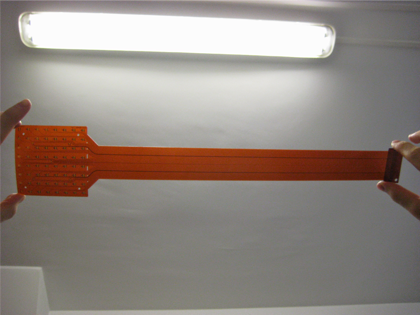
\includegraphics[width=.4\textwidth]{img/KDBWithPigTail.png}
    	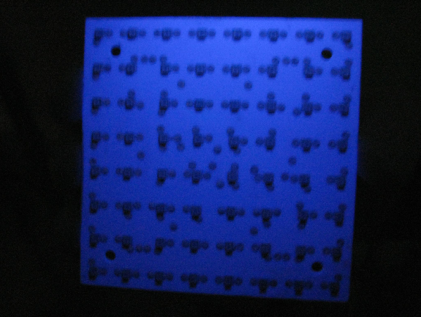
\includegraphics[width=.4\textwidth]{img/DC2.png}
	\caption{\label{fig.DB} Dice boards developed by the NEXT experiment. (a) Each DB provides 64 circuits and a long pig tail to transport the signals. (b) Response of a DB (emitting blue light) when illuminated with a UV lamp.}
\end{figure}

{\bf The technology transfer}, from the NEXT experiment (the main project of the PI, awarded with an AdG/ERC) to the PETALO spinoff. The NEXT tracking plane uses SiPMs arranged in matrices coated with TPB (Figure \ref{fig.DB}), which are the basis of the LXSC. The expertise and know-how acquired by the PI team both in the use of SiPMs and in the coating techniques with TPB will be directly applied to PETALO.

\newpage
\section*{\bf \textsf{Section 2 --Expected Impact (max 2 pages)}}

\subsection*{a. Economic and/or societal benefits}

The main application of PET to medicine is oncology, and, in recent years, neuroimaging. The oncological applications are mostly based in the use of FDG, a glucose analog where an atom of fluorine-18 (F-18) replaces an atom of oxygen. FDG-PET can be used for diagnosis, staging, and monitoring treatment of many types of cancer. The technology is also very well suited to search for tumor metastasis, or for recurrence after a known highly active primary tumor is removed. 

A typical dose of FDG used in an oncological scan has an effective radiation dose of 14 mSv, equivalent to about 5 years of dose by background radiation (combining natural and artificial sources). It follows that one of the important issues in PET applications is to reduce the FDG dose as much as possible, which, in turn requires an axial coverage as large as possible. Today's scanner have axial lengths of 15-25 cm. A larger scanner improves the solid angle, resulting in a larger acceptance and therefore allowing a dose reduction. Unfortunately {\bf the cost of current PET scanners is very high}, limiting their dimensions, and in particular its axial length. The fact that  individual PET scans are more expensive than ``conventional'' imaging with computed tomography (CT) and magnetic resonance imaging (MRI) limits also their use in clinical diagnose. {\bf Reducing costs of PET scanners is, therefore, a major priority to facilitate the expansion of the technology}. Conversely, the combination of PET with CT and MRI often leads to much improved scans, since the structural information offered by CT and MRI can be combined with the functional information offered by PET. 

PET neuroimaging uses the fact that the brain is an avid user of glucose, and since brain pathologies such as Alzheimer's disease greatly decrease brain metabolism of glucose standard FDG-PET of the brain, which measures regional glucose use, may also be successfully used to differentiate Alzheimer's disease from other dementing processes, and also to make early diagnosis of Alzheimer's disease. Neuroimaging requires images as clear as possible, and therefore high--performance PET scanners fully compatible with MRI (thus capable of operating in very intense, highly variable magnetic fields). Using time-of-flight (TOF) information is one of the best ways of boosting performance, insofar as the sensitivity of the scanner improves with $D/CTR$~, where $D$~is the diameter of the object being imaged (e.g, the head). An order of magnitude improvement in sensitivity can be reached by using
A PETALO scanner with a CTR of 100 ps. 

A PETALO scanner intended as a large acceptance ``full body'' PET, of $\sim$ 50 cm axial length and some 60-80 cm diameter could be build stacking 10 rings, each one made of about 40 large cells of $5 \times 5 \times 5$~cm$^3$~with (relatively) sparse SiPM instrumentation (32 SiPM per face, for a total of 64 SiPM per LXSC). The scanner would have lower cost and better sensitivity (due to the much improved CTR) than a LYSO scanner.  and  allows to reduce the number of random coincidences and permits TOF extrapolation, which in turn improves dramatically the scanner sensitivity. The reduced cost opens up the possibility of building a scanner with larger axial coverage (e.g, 50 cm to be compared with 25 cm for the larger LYSO devices), or to reduce the overall cost of the scanner. Furthermore, the costs of the sensors and electronics keeps dropping as the technology improves, while the cost of the LYSO crystals will not likely decrease due to the sophisticated manufacturing process involved. It follows that the relative cost of the PETALO technology with respect to LYSO scanners will improve in favor of PETALO in the next few years. 

\begin{framed}
Thus, PETALO has the potential to offer PET scanners {\bf with improved performance and significant reduced cost}, with respect to the current state-of-the-art.
\end{framed}

A PETALO scanner intended for neuroimaging can be based in trapezoidal cell (truncated pyramids) for better coverage and can increase the number of SiPMs (to 128) to optimise the energy resolution and the spatial resolution, while aiming to a  CTR  better than 100 ns. Such a device would be a true break-through with respect to the state-of-the-art in brain scanners. 

Last but not least, the PETALO technology is expected to be fully compatible with MRI, thus making it suitable for combined MRI-PET scanners. 

%To conclude, PETALO offers the potential to reduce the costs of PET scans, making the technology more accesible in clinical applications, in particular in oncology. Alternatively, it is possible to design large-acceptance (``full body'') PETALO scanners capable to reduce the exposition time and/or the dose to the patient. At the same time, the excellent energy resolution, very good spatial resolution in the three coordinates and excellent CRT results in a high performance scanner, which, combined for some applications with MRI can raise up the current standards in applications such as neuroimaging which are becoming an increasingly important tool in the study of the brain as well as in the diagnose of pathologies such as Alzheimer. 


\subsection*{b. Commercialisation process and/or any other exploitation process} 
A patent, held by CSIC and University of Valencia, with the PI as inventor, has been requested, protecting the idea of the LXSC, in view of future commercial applications.

This PoC requests funding to build a demonstrator scanner of dimensions and performance suitable for neuroimaging studies using state-of-the-art brain phantoms\footnote{{\em Three-dimensional brain phantom containing bone and grey matter structures with a realistic head contour}, Ann Nucl Med (2013) 27:25--36} . The time frame of PoC projects is sufficient to construct the demonstrator, characterise its performance and assess its potential as clinical device and research tool for brain studies. The studies will include a full characterisation of the scanner sensitivity, energy and spatial resolution, CTR and MRI compatibility, using standard phantoms. Therefore, the proposed outcomes (deliverables) of this PoC are: {\bf a technical report}, describing the construction of the scanner and its performance and a {\bf a conceptual design report}, assessing the feasibility and costs, of clinical devices, in particular of a large scanner suitable for oncology applications and a scanner for neuroimaging. 

Further steps could include: a) the construction of a large PETALO scanner, financed by public and/or private research funds (e.g, a join venture between a university consortium including university hospitals with teams experts in the clinical use of PET and companies interested in the application, such as Phillips, Siemens, etc.). b) The launching of an startup technological company to fabricate and commercialise PETALO scanners and/or c) the acquisition of the technology by one of the larger PET manufacturers. 
\newpage

\section*{\bf \textsf{Section 3 --The proof of concept plan (max 2 pages)}}

We propose to build a demonstrator of PETALO consistent in a  scanner of 23 cm internal diameter and 26 cm external diameter, with an axial length of 3 cm. Those dimensions are suitable to demonstrate good spatial and energy resolution and to show a large gain when using TOF information. 
The radial dimensions of the demonstrator are also appropriated  for neuroimaging studies using brain phantoms. After successfully demonstrating the concept, the axial coverage of the scanner can be incremented, to 15-21 cm by assembling together several rings. 
 
The ring is formed by assembling 22 LXSCs whose shape is a truncated pyramid, to guarantee maximum packing. The entry face of the cell (relative to the gammas line of flight) is a square of $3.0 \times 3.0$~cm$^2$ and the exit face of the cell is a square of  $4.0 \times 4.0$~cm$^2$. The depth is 3 cm, so that 60\% of the incoming 511 keV gammas interact in the cell.
The DBs are equipped with long pig tails that are connected to feedthroughs located in the back of the cryostat.  The signals from the SiPMs are amplified by the TOFPET ASIC, v2, fabricated by PETSYS. The ASIC design is intended to optimise both energy and CTR resolution. 

The ring has 1342 SiPM channels (61 per LXSC). PETSYS provides 128 channels front-end-boards (FEB). A total of 11 FEBs are needed for the whole scanner. The system provided by PETSYS includes firmware and DAQ software. The availability of commercial, off-the-shell, state-of-the-art ASIC electronics optimised for TOF resolution and at a very competitive price (25 \euro per channel) simplifies and speeds the development of this project.  


\subsection*{a. Plan of the activities}
{\bf Development of the activities}. A Gantt chart summarising the development of activities is shown in (Figure \ref{fig.pmp}). 

\begin{figure}[!htb]
	\centering
	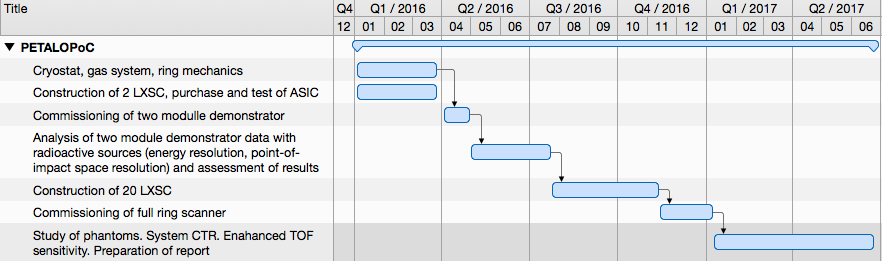
\includegraphics[width=.8\textwidth]{img/pmp.png}
	\caption{\label{fig.pmp} Gantt chart for the development of the PETALO demonstrator.}
\end{figure}
The plan of the activities is detailed in Figure \ref{fig.pmp} and can be briefly summarised as follows: 

{\bf Cryogenics, gas system and mechanics}.
The first step in the development of the project will be the construction of a cryostat, consisting on a cylinder of 22 cm inner diameter, 25 cm outer diameter, and 25 cm height suitable to support up to 8 PETALO rings.  The cryostat will be equipped with a cold head to liquify the xenon gas, and will be connected to a small system to recirculate, purify and recover the gas. It will be be built with diamagnetic stainless steel, to guarantee compatibility with MRI. The surfaces corresponding to the entry faces of the LXSCs will be covered with mylar windows. 

{\bf Construction, operation and analysis of a two-module system}. In parallel with the construction of the cryostat (3 months) 2 LXSC will be built.  Once the cryostat is ready, the two LXSCs will be placed in the ring facing each other and the system will be commissioned. Calibration tests will be run with a source of Na-22 providing back-to-back 511 keV photons and located in the center of the field-of view (FOV). The test will allow the measurement of the energy resolution of the individual LXSCs, the resolution in the impact point of the gammas, and the CTRs obtained from the reconstruction of a large number of lines-of-response (LORs) between the two modules. 

{\bf Construction, operation and analysis of the full system}. The remaining 20 LXSCs will be built and the whole system will be installed in the ring and commissioned. The characterisation of the full system will be done first with radioactive sources (Na-22) and then with standard phantoms, in particular with state-of-the-art brain phantoms, in order to determine the effective PET sensitivity, which will be measured with and without TOF analysis. 

\subsection*{b. Project-management plan}
The project management plan (PMP) controls: a) the development of the activities, already described ; b) the resources allocated to the activities; c) the logistics of the project including interaction with suppliers; d) the preparation and publication of scientific report(s).

The activities will be organised in three major working packages (WP): 

{\bf WP1: mechanics}. This activities of this package will include the construction of 
the cryostat and the ring mechanics,  the construction of the gas system,  and the construction of the LXSCs, including the feedthroughs needed to extract the signals. 

{\bf WP2: electronics and DAQ}. This package coordinates the acquisition and testing of SiPMs, the construction and coating with TPB of dice boards, the acquisition and testing of the ASIC FEBs and the commissioning of the whole electronics chain. 

{\bf WP3: software and analysis}. Includes the development of a full Monte Carlo simulation of the demonstrator and the development of the needed software tools and analysis program. 

{\bf Results}. The main result of the PoC is the characterisation of: a) the performance of the LXSCs, showing a resolution of around 12 \% FWHM, a transverse spatial resolution (1--2 mm) comparable with that of the finely segmented LYSO systems, and a longitudinal resolution (1 mm) much better than LYSO scanners; b) the study of the performance of the whole system, in particular the CTR of the system, which we expect better than 100 ps FWHM; c) the application of TOF information to increase the sensitivity of the whole system; d) the proof of the technical feasibility of the system; e) the assessment of the costs and technical issues associated with the construction of clinical devices. 

The project will make extensive use of the infrastructures and technological developments already achieved by the NEXT project. In particular, the cryostat will be fabricated by the same specialised company that has developed the vacuum/pressure chambers of NEXT, the gas system will reuse the components available from NEXT prototypes, The dice boards and feedthroughs of the LXSCs will be straight-forward modifications of those developed for the NEXT-100 detector, and the project will also reuse the software and Monte Carlo simulation tools developed by NEXT. 

\subsection*{c. Description of the team}
The team will include: {\bf The PI}, who will supervise the project. {\bf A project manager, PM} (Prof. José F. Toledo), who will follow the technical aspects and day by day development of the project and will also seek potential partners. {\bf A mechanical engineer} (A. Martínez), who will lead the activities of WP1. {\bf Two electronic engineers} (J. Rodriguez, V. Alvarez) working in WP2. {\bf A post-doc} who will work in WP3 (Dr. J. Renner), and one graduate student (J.M. Benlloch) who has already completed a Master Thesis in working in the simulation studies which have lead to this PoC and will take part in most of the activities of the project (including commissioning of detectors and scanner, tests of sensors and electronics, simulation, operation of the system and data analysis). In addition, the PI has established a collaboration with two groups of specialists in PET. The GIBI230 group, working at the hospital La Fe (Valencia), led by the prestigious radiologist Dr. Luis Marti-Bonmati\footnote{url{http://www.iislafe.es/biomedica-imagen.aspx}}, and the PET group at the
Institute of Neuroscience and Medicine in Juelich (Germany), lead by Dr.  Christoph Lerche\footnote{url{http://www.fz-juelich.de/inm/inm-4/EN/Forschung/PET-Physik/\_node.htm}}. The GIBI230 group will provide support for the tests of compatibility of PETALO with MRI using a research MRI device available at the hospital and will help the PI and the PM in the evaluation of clinical applications. The Juelich PET group specialises in neuroimaging and will provide expert help in this area (in particular in the use of brain phantoms).

\newpage

\section*{\bf \textsf{Section 4 --The budget (max 1 page + costing table)}}

The budget is almost entirely devoted to the construction of the scanner. The three engineers in the team are IFIC staff, and their activities will be covered by IFIC at no cost for this project. The Ph.D. student has a 4 years fellowship, also independent of this project, and the post-doc is supported by a Fulbright Fellowship. Both the PI and the PM are faculty. 

The cost of the scanner is easily described in terms of:
\begin{enumerate}
\item {\bf Mechanics}, including the cryostat (20,000 \euro), the support ring, construction of the LXSC boxes, as well as vacuum and cryogenic equipment (10,000 \euro).
\item {\bf The LXSCs}: each module costs 3,668 \euro (Table \ref{tab.box}). The 22 modules cost 80,696 \euro. 
\item {\bf Travel}, needed to visit companies (suppliers as well as potential partners) as well as attending meetings with collaborators (e.g, the Julich group) and at least one conference. We estimate 9,000 \euro, around 3,000 \euro\ for the PI and 6,000 \euro\ for the rest of the team. 
\end{enumerate}

The project will benefit from the infrastructure available at IFIC. It will be developed in the NEXT laboratory, and fully profit from the NEXT and IFIC electronics and mechanics workshops. The gas system, vacuum pumps, small electronics components and electronics equipment will be available from the NEXT equipment, as well as the computers needed for the DAQ (which will use the same protocol, called DATE, used by NEXT).  

\begin{table}[htdp!]
\caption{Cost of each LXSC}
\begin{center}
\begin{tabular}{|c|c|}
\hline
item & cost (\euro) \\
\hline
xenon &	113 \\
SiPMs &	1830 \\
ASIC	 & 1525 \\
Dice Board & 100 \\
Mechanics &100 \\
\hline
Total	 & 3668 \\
\hline\hline
\end{tabular}
\end{center}
\label{tab.box}
\end{table}%

\begin{table}[htdp!]
\caption{Budget}
\begin{center}
\begin{tabular}{|c|c|}
\hline
Category & Cost (in \euro) \\
\hline
Equipment & 110,698 \\
Travel & 9,000 \\
Total direct costs & 119,698 \\
25 \% of direct costs & 29,924 \\
Total requested EU contributions & 149,623 \\
\hline\hline
\end{tabular}
\end{center}
\label{tab.box}
\end{table}%
 

\end{document}